\subsection{Longest-Chain Protocols are Timely}

We now prove that longest-chain protocols are timely both in proof-of-work and proof-of-stake.
For concreteness, we work in the Bitcoin Backbone setting
as a representative of proof-of-work and in the Ouroboros setting
as a representative of proof-of-stake.
Regardless, we work with abstract chain virtues
and show that any longest-chain
temporal blockchain protocol with Common Prefix,
Chain Quality and Chain Growth is timely,
provided it has consistent recorded rounds.
In this subsection, we are in the 
static synchronous setting with $\Delta = 1$.

\begin{definition}[Longest-Chain Protocol]
  A longest-chain protocol with confirmation parameter $k$
  is a blockchain protocol for which,
  at the beginning of any round $r$, every honest party $P$ \emph{adopts}\footnote{
    At the beginning of a round $r$, before observing the network, we say that
    honest party $P$ \emph{has} an unstable chain $\HChain[][P][r]$ (this chain
    contains any block honestly generated by $P$ at the previous round), whereas
    upon observing the network, the honest party \emph{adopts} the longest
    valid unstable chain $\TChain[][P][r]$.
  }
  the \emph{longest} valid observed unstable chain $\TChain[][P][r]$. It outputs the
  chain $\Chain[][P][r] = \TChain[][P][r][:-k]$.
  Honest parties always generate blocks that extend their adopted unstable chain.
\end{definition}

We first prove freshness.
For the notation definitions ($\mu, \ell, \tau, s$)
in the following theorem, refer to the original Bitcoin
Backbone paper~\cite{backbone-new}.

\begin{theorem}[Longest-Chain Freshness]
  Temporal Blockchains, following the longest chain rule,
  with \emph{Chain Quality($\mu,\ell$)},
  %, Common Prefix($k$),
  \emph{Chain Growth($\tau, s$)},
  and consistent recorded rounds
  are fresh with parameter $w =\max(s, \frac{k + \ell}{\tau}) + 1$.
\end{theorem}
\begin{proof}
  Let $P$ be any honest party and $r$ be any round.
  Suppose, towards a contradiction, that block $B^*$
  is the tip of finalized chain $\Chain[][P][r]$ and has
  recorded round $r^* < r - w$.

  Let $B'$ be the most recent honestly generated block
  in $\Chain[][P][r][{-\ell}{:}]$.
  (or let $B'$ be genesis if $|\Chain[][P][r][{-\ell}{:}]| \leq \ell$).
  This block exists by
  Chain Quality because we are looking at a chain chunk of length at least $\ell$ and
  $\mu\ell \geq 1$ (or is genesis).
  Let $r'$ be the round in which $B'$ was generated.
  Its recorded round is also $r'$.
  Let $P'$ be the party who generated $B'$
  (or $P' = P, r' = 0$ if $B'$ is genesis).
  Block $B^*$ extends a chain that contains $B'$, so $r^* \geq r'$,
  therefore:
  \begin{equation}
    r' < r - w \label{eq:bitcoin-r-bound}
  \end{equation}

  Let $\TChain[][P'][r']$ be the chain that $P'$ adopts at
  round $r'$ (this will be the empty chain if $B'$ is genesis).
  Party $P'$ extends $\TChain[][P'][r']$, at round $r'$, with block $B'$,
  creating a chain of length $|\TChain[][P][r']| + 1$.
  This newly generated chain is broadcasted to the network and
  received by party $P$ at the beginning of round $r' + 1$.
  Let $\HChain[][P][r' + 2]$ be the chain
  that $P$ \emph{has} at round $r' + 2$.
  We observe that, at round $r' + 2$, due to the
  longest chain rule, party $P$ \emph{has} a chain of greater or equal
  length to the one broadcasted by party $P^*$. Hence
  $|\HChain[][P][r' + 2]| \geq |\TChain[][P'][r']| + 1$. Therefore:

  \begin{equation}
    |\TChain[][P][r]| - |\HChain[][P][r' + 2]| \leq
     |\TChain[][P][r]| - |\TChain[][P'][r']| - 1 <
     k + \ell\, \label{eq:bitcoin-contradiction}
  \end{equation}

  For the second inequality, refer to Figure~\ref{fig:longest-chain-freshness-proof}
  % observe that
  % $\TChain[][P][r][{:}-k]$ is the chain with block $B^*$ as tip,
  % whereas $\TChain[][P'][r']$ is the parent chain of block $B'$.
  % Those are spaced at most $\ell$ blocks apart by the definition of $B'$.

  \begin{figure}
    \centering
    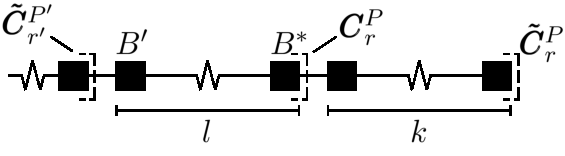
\includegraphics[width=0.45\columnwidth,keepaspectratio]{figures/longest-chain-proof.pdf}
    \caption{Longest-Chain blockchains freshness proof. For the position of $B'$ we illustrate the
             earliest possible.
    }
   \label{fig:longest-chain-freshness-proof}
  \end{figure}


  On the other hand, by Inequality~\ref{eq:bitcoin-r-bound}, $r - (r' + 2) \geq w - 1 \geq s$ and
  we can apply Chain Growth between rounds $r' + 2$ and $r$
  with parameters $s, \tau$ to obtain
  $|\TChain[][P][r]| - |\HChain[][P][r' + 2]| \geq \tau(r - (r' + 2)) \geq \tau (w - 1) =  k + \ell$,
  which is a contradiction because of Inequality~(\ref{eq:bitcoin-contradiction}).
  \Qed
\end{proof}

We now make a couple of small changes to the Bitcoin and Ouroboros
construction to turn them into Temporal Blockchains.
Our changes correspond to the real Bitcoin and Ouroboros deployments, in which timestamps (recorded rounds)
are included in the block
% TODO(dionyziz): replace this citation with a reference to the original Nakamoto client commit that introduced timestamps to the header
headers~\cite{mastering-bitcoin}. \atnote{Add citation for Ouroboros as well.}

\noindent
\textbf{Temporal Bitcoin.}
Our Temporal Bitcoin construction is illustrated in Figure~\ref{fig.temporal-backbone}.
It is clear that the Temporal Bitcoin construction retains the properties of Common Prefix,
Chain Quality and Chain Growth proven in the original Bitcoin Backbone paper~\cite{backbone}.
The reason is that the only change we make is to add a round number to the block format, and
the validity predicate of an honestly produced block is unaffected by the new validity rules.
Furthermore, it has consistent recorded rounds.

\begin{figure}
  The Temporal Bitcoin protocol is the Bitcoin protocol with
  the following additions:

  \begin{enumerate}
    \item Blocks include a round number.
    \item Genesis has recorded round $0$.
    \item Honest parties mine blocks with the current round.
    \item When a chain is received by an honest party, we add the following validity rules:
          \begin{enumerate}
            \item Recorded rounds are strictly increasing.
            \item Recorded rounds are not in the future.
          \end{enumerate}
  \end{enumerate}
  \caption{Temporal Bitcoin construction.}
  \label{fig.temporal-backbone}
\end{figure}

\noindent
\textbf{Temporal Ouroboros.}
The Temporal Ouroboros protocol is the Ouroboros protocol with
the following additions: No future slot blocks are accepted.
In each block, we report $??? e$ \atnote{Fill this in} as the recorded round, where $e$ is its slot.
\atnote{In Ouroboros they use $r$ for slot.}
Temporal Ouroboros retains the properties of Common Prefix,
Chain Quality and Chain Growth proven in the original Ouroboros paper~\cite{ouroboros}.
Furthermore, it has consistent recorded rounds.

We observe that for all longest-chain protocols, safety follows from the
Common Prefix property. Hence, from the above and Theorem~\ref{thm:freshness-to-timeliness},
it follows that Temporal Bitcoin and
Temporal Ouroboros are timely with parameter $v = \max(s, \frac{k + \ell}{\tau}) + 1$.

% \begin{theorem}[Bitcoin Timeliness]
%   A typical execution of the Temporal Bitcoin Backbone protocol is timely
%   with timeliness $v = \max(s, \frac{k + \ell}{\tau}) + 1$.
% \end{theorem}
% \begin{proof}
%   Requirements (1) and (2) of timeliness are satisfied due to the new chain validity rules.
%   We will now prove (3).
%
%   Let $P$ be any honest party and $r_1 \leq r_2 \in \mathbb{N}$ be any rounds, and consider
%   the ledgers $\Ledger[][P][r_1], \Ledger[][P][r_2]$ reported\footnote{
% Recall that the ledger reported at a round is obtained by inspecting the
%     chain \emph{adopted} at that round.
%   } by $P$ at rounds $r_1, r_2$ respectively.
%   Suppose, towards a contradiction, that $\Ledger[][P][r_2][|\Ledger[][P][r_1]|{:}]$ contains a transaction
%   $\tx$ with recorded round $r \leq r_1 - v$.
%
%   % TODO(dionyziz): figure
%   Let $\chain_1, \chain_2$ be the chain that $P$ adopts at round $r_1$
%   and $r_2$ respectively.
%   It must be true that $|\chain_2| > |\chain_1|$.
%   Due to Common Prefix, $\chain_2$ will extend a block in $\chain_1[-k-1{:}]$.
%   The transaction $\tx$ is contained in some block $B$ of $\chain_2[|\chain_1[{:}{-k}]|{:}{-k}]$.
%
%   Let $B^*$ be the most recent
%   honestly generated block in $\chain_1[{:}{-k}][{-\ell}{:}]$
%   (or let $B^*$ be genesis if $|\chain_1| \leq \ell + k$).
%   This block will exist by
%   Chain Quality because we are looking at a chain chunk of length at least $\ell$ and
%   $\mu\ell \geq 1$ (or is genesis).
%   Block $B^*$ is honestly generated, so let $r^*$ be the round
%   during which $B^*$ was generated, noting that the round recorded in $B^*$ is $r^*$.
%   Let $P^*$ be the party who mined $B^*$ at round $r^*$ (or $P^* = P, r^* = 0$ if $B^*$ is
%   the genesis block).
%
%   The block $B$ extends a chain that contains $B^*$, so $r > r^*$,
%   therefore
%   \begin{equation}
%     r^* < r_1 - v\label{eq:bitcoin-r-bound}.
%   \end{equation}
%
%   Let $\chain^{P^*}_{r^*}$ be the chain that $P^*$ adopts at
%   round $r^*$ (this will be the empty chain if $B^*$ is genesis).
%   Party $P^*$ extends $\chain^{P^*}_{r^*}$, at round $r^*$, with block $B^*$,
%   creating a chain of length $|\chain^{P^*}_{r^*}| + 1$.
%   This newly generated chain is broadcasted to the network and
%   received by party $P$ at the beginning of round $r^* + 1$.
%   Let $\bar \chain^P_{r^* + 2}$ be the chain
%   that $P$ \emph{has} at round $r^* + 2$.
%   We observe that, at round $r^* + 2$, due to the
%   longest chain rule, party $P$ \emph{has} a chain of greater or equal
%   length to the one broadcasted by party $P^*$. Hence
%   $|\bar \chain^P_{r^* + 2}| \geq |\chain^{P^*}_{r^*}| + 1$. Therefore
%
%    % This is also the chain that $P$ \emph{has} at round $r^* + 2$.
%
%   \[
%      |\chain_1| - |\bar \chain^P_{r^* + 2}| \leq
%      |\chain_1| - |\chain^{P^*}_{r^*}| - 1 <
%      k + \ell\, \label{eq:bitcoin-contradiction}\tag{$\ast$}.
%   \]
%
%   For the second inequality, observe that
%   $\chain_1$ is the chain of $P$ adopted at round $r_1$,
%   whereas $\chain^{P^*}_{r^*}$ is
%   the parent chain of $B^*$ and those are spaced at most $k + \ell$ blocks
%   apart by the definition of $B^*$.
%
%   On the other hand, by Equation~\ref{eq:bitcoin-r-bound}, $r_1 - (r^* + 2) \geq v - 1 \geq s$ and
%   we can apply Chain Growth between rounds $r^* + 2$ and $r_1$
%   with parameters $s, \tau$ to obtain
%   $|\chain_1| - |\bar \chain^P_{r^* + 2}| \geq \tau(r_1 - (r^* + 2)) \geq \tau (v - 1) \geq
%   \tau (\frac{k + \ell}{\tau} + 1 - 1) \geq k + \ell$,
%   which is a contradiction because of Equation~(\ref{eq:bitcoin-contradiction}).
%
%   \Qed
% \end{proof}


% \subsection{Ouroboros Proof-of-Stake}
% \dznote{Prove that Ouroboros is timely}
